\documentclass[9pt]{beamer}

\usepackage[T1]{fontenc}
\usepackage{color}
\usepackage{graphicx}
\usepackage{natbib}
\usepackage{tikz}
\usepackage{pgfgantt}
\usepackage{booktabs}
\usepackage{framed}

\usetheme{Boadilla}

\definecolor{rd}{HTML}{2F2A40}
\definecolor{methods}{HTML}{C6C6C6}
\definecolor{research}{HTML}{8F84BE}
\definecolor{skills}{HTML}{7A7A7A}
\definecolor{rc}{HTML}{AC152A} 

\usefonttheme{professionalfonts}

\title[Climate Topography]{A Topography of Climate Change Research}
\subtitle{}
\author{Max Callaghan}
\institute[MCC]{
	
\includegraphics[height=1cm,width=2cm]{MCC_Logo_RZ_rgb.jpg}
%	\,
%	
\includegraphics[height=1cm]{hertie_logo.png}
}

\newtheorem*{remark}{}

\bibliographystyle{apalike}

\begin{document}
	
\begin{frame}
	\titlepage
\end{frame}

\addtobeamertemplate{frametitle}{}{%
	\begin{tikzpicture}[remember picture,overlay]
	\node[anchor=north east,yshift=2pt] at (current page.north east) {
\includegraphics[height=0.8cm]{MCC_Logo_RZ_rgb.jpg}};
	\end{tikzpicture}}

\begin{frame}{Context}

\begin{columns}
	\begin{column}{0.5\linewidth}
		\begin{center}
		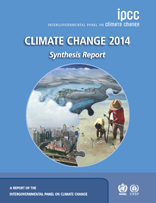
\includegraphics[width=0.6\linewidth]{syrcover.png}
		\end{center}
	\end{column}
	\begin{column}{0.5\linewidth}
	\begin{center}
		\begin{itemize}
			\item To contribute evidence-based policy-making on climate change, the IPCC aims to \textit{comprehensively} assess  
			\item These assessments should be aim to balance legitimacy, credibility and relevance \citep{Cash2001}
		\end{itemize}
	\end{center}
	\end{column}
	\end{columns}

\end{frame}

\begin{frame}{Motivation}

\begin{columns}
	\begin{column}{0.5\linewidth}
		\begin{figure}
		\includegraphics<1>[width=1\linewidth]{../plots/volume_variety_AR0}
		\includegraphics<2>[width=1\linewidth]{../plots/volume_variety_AR1}
		\includegraphics<3>[width=1\linewidth]{../plots/volume_variety_bible_AR1}
		\includegraphics<4>[width=1\linewidth]{../plots/volume_variety_bible_AR2}
		\includegraphics<5>[width=1\linewidth]{../plots/volume_variety_bible_AR3}
		\includegraphics<6>[width=1\linewidth]{../plots/volume_variety_bible_AR4}
		\includegraphics<7>[width=1\linewidth]{../plots/volume_variety_bible_AR5}
		\includegraphics<8->[width=1\linewidth]{../plots/volume_variety_bible_AR6}
		\end{figure}
	\end{column}
	\begin{column}{0.5\linewidth}
		\begin{center}
		\only<1>{\framebox[1.1\width]{A matrix of documents x words } \par}
		\only<2>{\framebox[1.1\width]{AR1: 1,848 documents x 3,528 words } \par}
		\only<3>{\begin{framed}
			The Luther Bible: 1,189 documents (chapters) x 11,973 words
			\end{framed}}
		%\only<3>{\framebox[1.1\width]{The Luther Bible: \par 1,189 documents (chapters) x 11,973 words } \par}
		\only<4>{\framebox[1.1\width]{AR2: 6,941 documents x 15,781 words } \par}
		\only<5>{\framebox[1.1\width]{AR3: 18,728 documents x 27,730 words } \par}
		\only<6>{\framebox[1.1\width]{AR4: 44,000 documents x 45,388 words } \par}
		\only<7>{\framebox[1.1\width]{AR5: 108,277 documents x 75,553 words } \par}
		\only<8->{\framebox[1.1\width]{AR6: 128,357 documents x 86,149 words } \par}
		\end{center}
		\only<9->{		
		\begin{center}
			\begin{itemize}
				\item Comprehensive, credible and relevant assessments become
				more challenging as the literature grows
			\end{itemize}
		\begin{remark}[]
			To understand, and to aid, scientific assessments of climate change, we need to machine read the literature
		\end{remark}
		\end{center}
	}
	\end{column}
\end{columns}

\end{frame}



\begin{frame}{Approach - Words, words, words}

\begin{columns}
	\begin{column}{0.5\linewidth}
		\begin{center}
			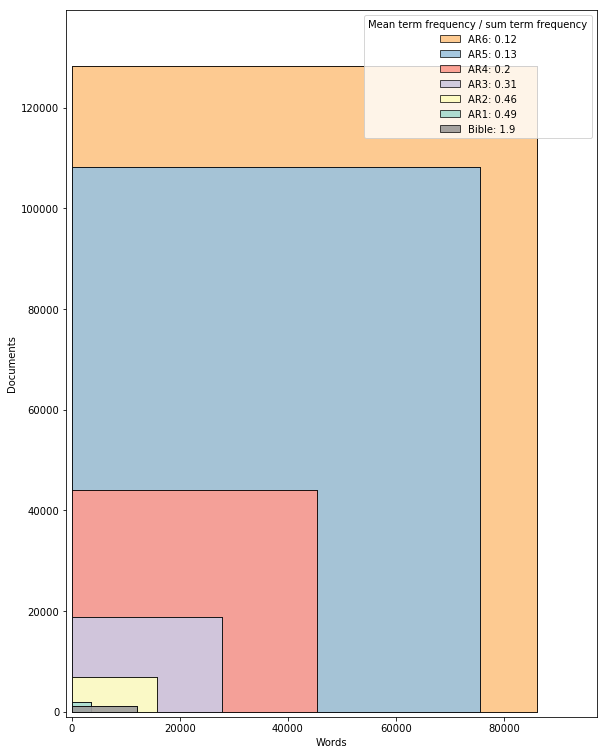
\includegraphics[width=\linewidth]{../plots/volume_variety_bible_AR6}
		\end{center}
	\end{column}
	\begin{column}{0.5\linewidth}
		\textbf{Topic Modelling}
		\begin{center}
			\begin{itemize}
				\item Topic modelling is a way of reducing the dimensionality of a corpus of documents
				\item A large matrix of documents x words is factorised by
				a matrix of topics x words and a matrix of topics x documents
			\citep{Lee1999}
				\item Topics describe the latent structure of the document corpus
				
			\end{itemize}
		\end{center}
	\end{column}
\end{columns}

\end{frame}

\begin{frame}{Approach - Words, words, words}

\begin{figure}
	
	\only<1>{\(V_{i\mu} \) is a term frequency-inverse document frequency matrix of \textit{stemmed} terms} 
	\only<2>{\[V_{i\mu} \approx (WH)_{i\mu} = \sum_{a=1}^{r}W_{ia}H_{a\mu} \]} %\(V\) is approximated by the product of \(W\) and \(H\)}
	
	\includegraphics<1>[width=\linewidth]{../plots/VWH_blank.png}
	\includegraphics<2>[width=\linewidth]{../plots/VWH}
	
	\only<1>{\caption{A topic model of 3495 documents on climate change from the year 2000}}
	
	\only<2>{\caption{A topic model of 3495 documents on climate change from the year 2000}}
	
\end{figure}

\end{frame}


%%%%%%%%%%%%%%%%%%%%%%%%

\begin{frame}{Research Questions}
\begin{columns}
	\begin{column}<1->{0.5\linewidth}
		\begin{framed}
			What is the thematic structure of the literature on climate change, and how has this changed over the five assessment periods of the IPCC
		\end{framed}
	\end{column}
	\begin{column}<2->{0.5\linewidth}
		\begin{framed}
			What can this modelled thematic structure tell us about the past and future relationship between the IPCC and scientific literature on climate change? 
		\end{framed}
	\end{column}
\end{columns}

\only<3->{
\textbf{Steps}
\begin{enumerate}
	\item Download documents from Web of Science (WoS)
	\item Match documents to reference lists from IPCC reports
	\item Topic model stemmed document abstracts
\end{enumerate}
}
\end{frame}

%%

\begin{frame}{Data - Query}
\begin{columns}
	\begin{column}{0.65\linewidth}
		\tiny
		(SO=(Climate Alert OR Climate Dynamics OR Climate Policy OR Climatic Change OR Global and Planetary Change OR Global Change Biology OR International Journal of Greenhouse Gas Control OR Mitigation and Adaptation Strategies for Global Change) OR TS=(((CO2 OR "carbon dioxide" OR methane OR CH4 OR "carbon cycle" OR "carbon cycles" OR "carbon cycling" OR "carbon budget*" OR "carbon flux*" OR "carbon mitigation") AND (climat*)) OR (("carbon cycle" OR "carbon cycles" OR "carbon cycling" OR "carbon budget*" OR "carbon flux*" OR "carbon mitigation") AND (atmospher*))) OR TS=("carbon emission*" OR "sequestration of carbon" OR "sequester* carbon" OR "sequestration of CO2" OR "sequester* CO2" OR "carbon tax*" OR "CO2 abatement" OR "CO2 capture" OR "CO2 storage" OR "CO2 sequester*" OR "CO2 sequestration" OR "CO2 sink*" OR "anthropogenic carbon" OR "captur* of carbon dioxide" OR "captur* of CO2" OR "climat* variability" OR "climat* dynamic*" OR "chang* in climat*" OR "climat* proxies" OR "climat* proxy" OR "climat* sensitivity" OR "climat* shift*" OR "coupled ocean-climat*" OR "early climat*" OR "future climat*" OR "past climat*" OR "shift* climat*" OR "shift in climat*") OR TS=("atmospheric carbon dioxide" OR "atmospheric CH4" OR "atmospheric CO2" OR "atmospheric methane" OR "atmospheric N2O" OR "atmospheric nitrous oxide" OR "carbon dioxide emission*" OR "carbon sink*" OR "CH4 emission*" OR "climat* policies" OR "climat* policy" OR "CO2 emission*" OR dendroclimatolog* OR ("emission* of carbon dioxide" NOT nanotube*) OR "emission* of CH4" OR "emission* of CO2" OR "emission* of methane" OR "emission* of N2O" OR "emission* of nitrous oxide" OR "historical climat*" OR IPCC OR "methane emission*" OR "N2O emission*" OR "nitrous oxide emission*") OR TS=("climat* change*" OR "global warming" OR "greenhouse effect" OR "greenhouse gas*" OR "Kyoto Protocol" OR "warming climat*" OR "cap and trade" OR "carbon capture" OR "carbon footprint*" OR "carbon neutral" OR "carbon offset" OR "carbon sequestration" OR "carbon storage" OR "carbon trad*" OR "changing climat*" OR "climat* warming")) NOT PY=2018
		
		\normalsize
		\begin{itemize}
			\item \citep{Haunschild2016}
			\item 309,697 documents
		\end{itemize}
	\end{column}
	\begin{column}{0.35\linewidth}
		\textbf{Caveats}
		\begin{itemize}
			\item Not perfect query
			\item WoS not all peer-reviewed literature
			\item Missing grey literature
			\item Missing relevant literature not directly about climate change
		\end{itemize}
	\end{column}
\end{columns}
\end{frame}

\begin{frame}{Methodology - Dynamic Topic Modelling}

The topic models above assume that the topics, and the words that make them up, are stable over time. Two approaches to better model dynamic topics:

\begin{itemize}
	\item<2->Dynamic Topic Modelling (DTM) \citep{Blei2006} assume that a constant number of topics exists over all topic models, but allows the words in the topics to evolve from one time period to another
	\item<3->Dynamic Non-negative Matrix Factorisation \citep{Greene2016} has varying numbers of topics in each window and allows for topics to emerge and/or disappear.
\end{itemize}

\onslide<4->{Where the size and variety of the literature we want to model has increased exponentially, we need an approach that allows for the emergence of new topics.}

\end{frame}

%%%%%%%%%%%%%%%%%%%%%%%
%% D-NMF


\begin{frame}[t]{Dynamic NMF}


\only<1->{
\includegraphics[]{C:/Users/galm/Documents/papers/sustainability/plots/VWH_1991}}
\only<2->{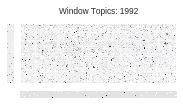
\includegraphics[]{C:/Users/galm/Documents/papers/sustainability/plots/VWH_1992}}

\only<3->{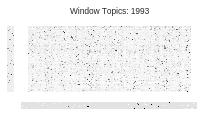
\includegraphics[]{C:/Users/galm/Documents/papers/sustainability/plots/VWH_1993}}

\end{frame}

\begin{frame}[t]{Dynamic NMF}

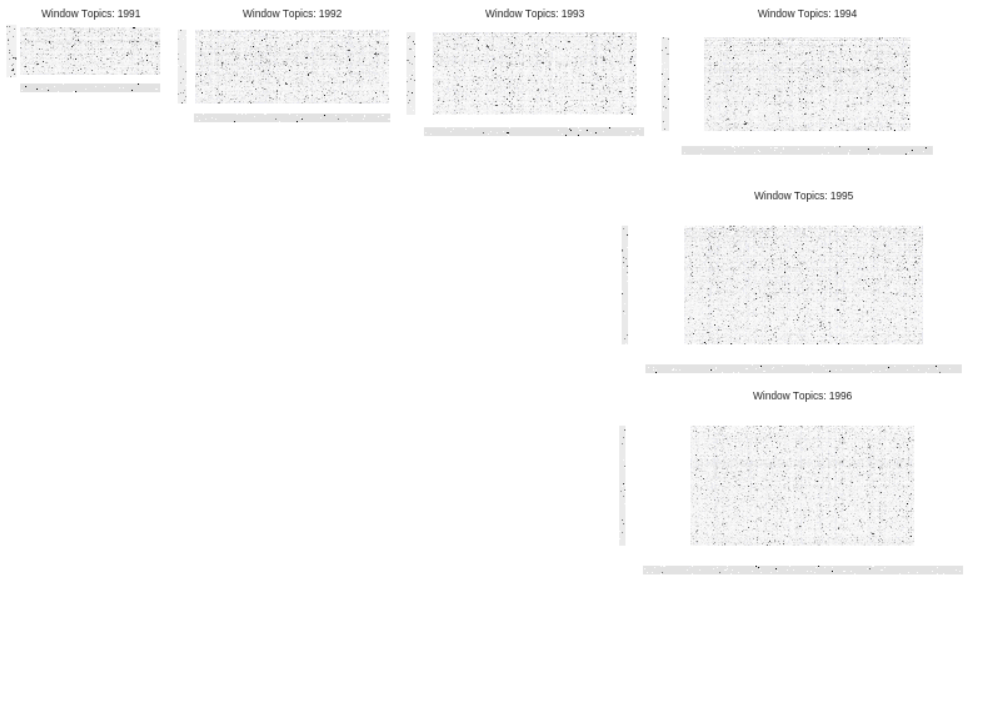
\includegraphics[width=\linewidth]{../plots/sustainability/conceptual_windows_only}

\end{frame}

\begin{frame}[t]{Dynamic NMF}

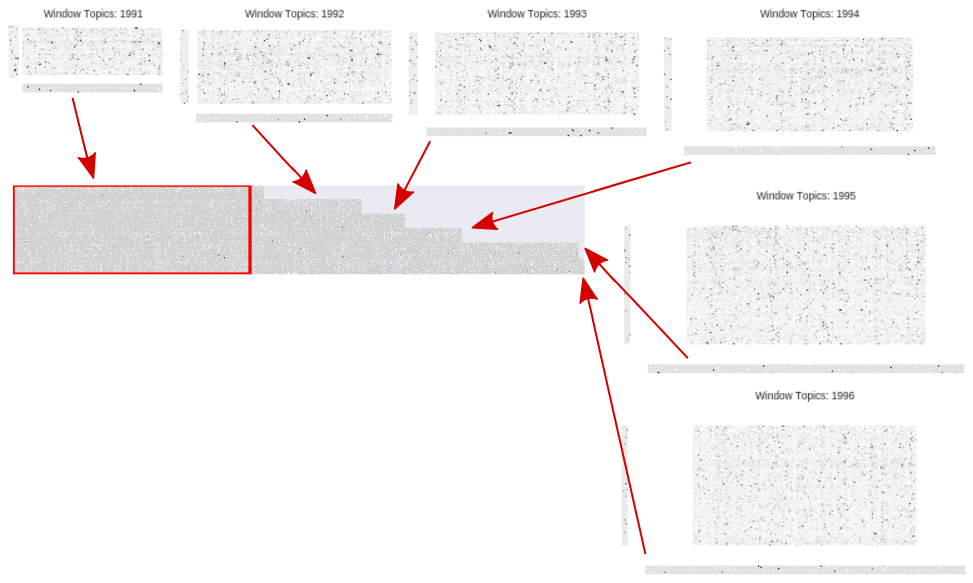
\includegraphics[width=\linewidth]{../plots/sustainability/conceptual_annotated_1}

\end{frame}

\begin{frame}[t]{Dynamic NMF}

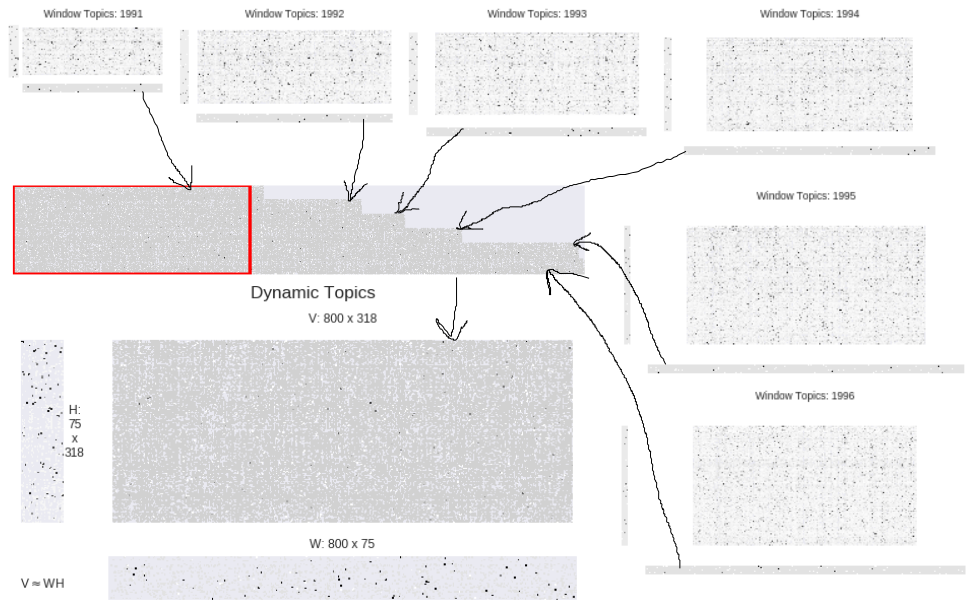
\includegraphics[width=\linewidth]{../plots/sustainability/conceptual_annotated_2}

\end{frame}


\begin{frame}{Dynamic NMF - application to climate change}

\onslide<1->{
\begin{itemize}
	\item Choosing the number of window topics is non-trivial. Data-driven approaches are limited (see below), and human selection is time consuming.
	\item To facilitate the description of trends over the assessment periods of the IPCC, and to minimize the number of modelling decisions, I consider each IPCC assessment period as a time window.
\end{itemize}}

\begin{columns}
	\onslide<2->{
	\begin{column}{0.5\linewidth}

			\begin{itemize}
				\item Starting from a logarithmic relationship between the number of documents and the ideal topic number, I compare 5 runs with varying numbers of topics for each window
		\end{itemize}
	\end{column}
	\begin{column}{0.5\linewidth}
		\begin{figure}
			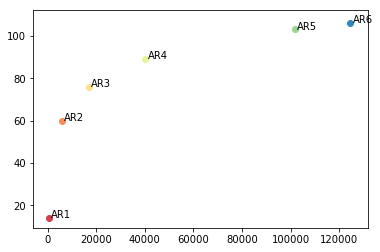
\includegraphics[width=\linewidth]{../plots/n_topics}	
		\end{figure}
	\end{column}
}
\end{columns}

\end{frame}





\begin{frame}[t]{Dynamic NMF - number of topics}

\begin{columns}
	\begin{column}{0.5\linewidth}
		\textbf{Human topic number criteria}
		\begin{itemize}
			\item Intelligibility
		\end{itemize}
		\textbf{Data-driven topic number criteria}
		\begin{itemize}
			\item Reconstruction accuracy
			\item Predictive capacity
		\end{itemize}
		\onslide<2->{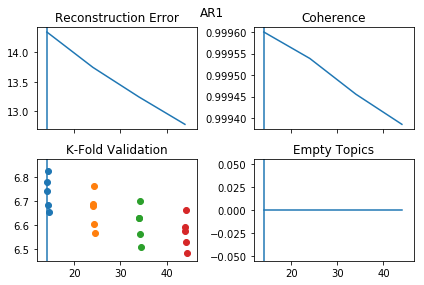
\includegraphics[width=0.8\linewidth]{../plots/topic_validations_AR1}}
	\end{column}
	\begin{column}<2->{0.5\linewidth}
		
\begin{figure}
	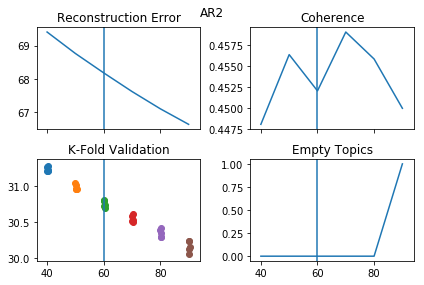
\includegraphics[width=0.8\linewidth]{../plots/topic_validations_AR2}
	
	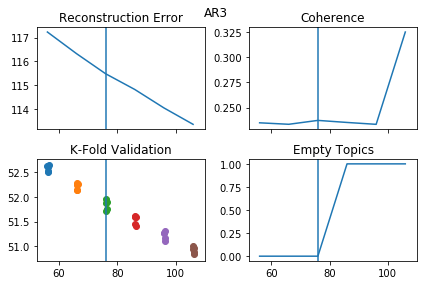
\includegraphics[width=0.8\linewidth]{../plots/topic_validations_AR3}
\end{figure}
	\end{column}
\end{columns}


\end{frame}


%%%%%%%%%%%%%%%%%%%%%%%%%%%%%%%%%%%
% results


%\begin{frame}{Preliminary results - explanation}
%
%\begin{columns}
%	\begin{column}{0.5\linewidth}
%		\begin{center}
%			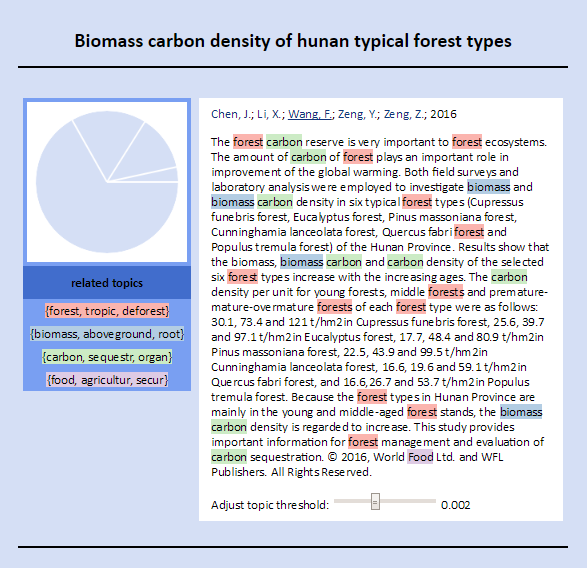
\includegraphics[width=\linewidth]{../plots/biomass_eg.png}
%		\end{center}
%	\end{column}
%	\begin{column}{0.5\linewidth}
%		\begin{center}
%			\begin{itemize}
%				\item Documents are mixtures of topics, based on the words which occur in them
%			\end{itemize}
%		\end{center}
%	\end{column}
%\end{columns}
%
%\end{frame}

%\begin{frame}{Preliminary results - Map}
%
%\begin{figure}
%			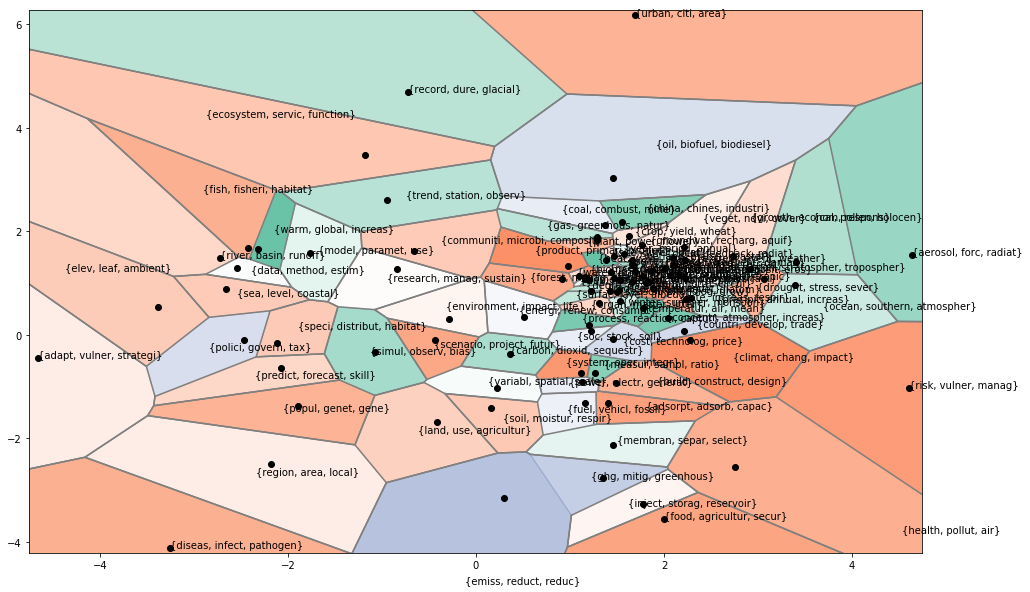
\includegraphics[width=\linewidth]{../plots/pca_map.png}
%			\caption{Topic Map, with topics placed according to Principal Component Analysis of topic-term matrix}
%\end{figure}
%
%\end{frame}


\begin{frame}{Preliminary results - structure}

\begin{columns}
	\begin{column}{0.65\linewidth}
		\begin{center}	
			\vspace*{-0.1\linewidth}
			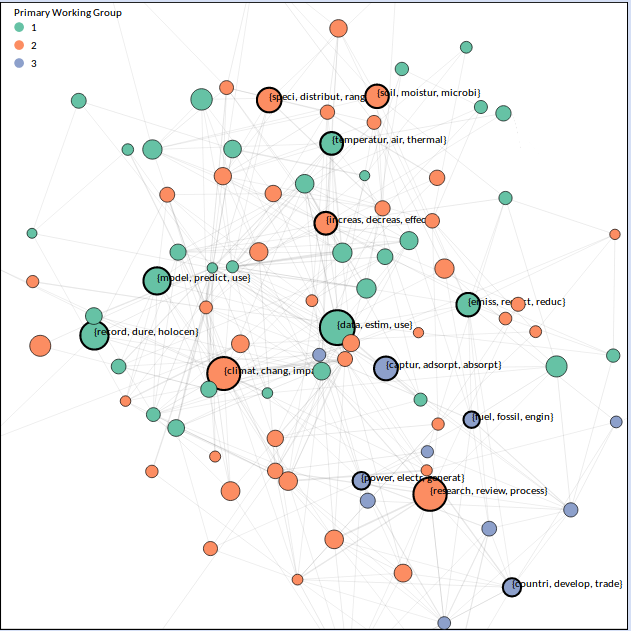
\includegraphics[width=\linewidth]{../plots/network_wg_654}
		\end{center}
	\end{column}
	\begin{column}{0.35\linewidth}
	%	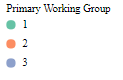
\includegraphics[width=0.4\linewidth]{../plots/network_wg_key}
		\begin{center}
			\begin{itemize}
				\item A network of comprehensible topics is generated with 100 topics
				\item Topics can be matched to the IPCC working group from which the majority of the topic documents are referenced in
				\item Topics from the same working group are \textbf{significantly} more likely to be correlated with each other than those which are not
			\end{itemize}
		\end{center}
	\end{column}
\end{columns}

\end{frame}


\begin{frame}{Preliminary results - Inter-working Group topics - WG 1 and 3}
	
	\begin{table}
		
		
		\begin{tabular}{p{1.4cm} p{1cm} l r r r}
\toprule
 IPCC Coverage &  Primary WG &               Topic Title &  WG 1 &  WG 2 &  WG 3 \\
\midrule
         0.16\% &           1 &  \{rainfal, monsoon, rain\} & 0.50\% & 0.50\% & 0.00\% \\
         0.10\% &           2 &      \{veget, ndvi, cover\} & 0.41\% & 0.59\% & 0.00\% \\
         0.16\% &           1 &     \{snow, cover, winter\} & 0.59\% & 0.41\% & 0.00\% \\
         0.17\% &           2 &    \{region, local, scale\} & 0.41\% & 0.59\% & 0.00\% \\
         0.16\% &           1 &  \{coastal, mangrov, rise\} & 0.57\% & 0.42\% & 0.01\% \\
\bottomrule
\end{tabular}

		
	\end{table}
	
\end{frame}

%%%%%%%%

\begin{frame}{Preliminary results - Inter-working Group topics - WG 1 and 3}
	
	\begin{table}
		
		
		\begin{tabular}{p{1.4cm} p{1cm} l r r r}
\toprule
 IPCC Coverage &  Primary WG &                   Topic Title &  WG 1 &  WG 2 &  WG 3 \\
\midrule
         0.09\% &           3 &        \{gas, coal, greenhous\} & 0.30\% & 0.15\% & 0.56\% \\
         0.10\% &           3 &     \{transport, vehicl, road\} & 0.24\% & 0.12\% & 0.64\% \\
         0.13\% &           1 &        \{emiss, reduct, reduc\} & 0.45\% & 0.21\% & 0.34\% \\
         0.09\% &           1 &  \{methan, oxid, methanotroph\} & 0.63\% & 0.16\% & 0.20\% \\
         0.13\% &           3 &         \{ghg, greenhous, gas\} & 0.15\% & 0.09\% & 0.75\% \\
\bottomrule
\end{tabular}

		
	\end{table}
	
\end{frame}

%%%%%%%

\begin{frame}{Preliminary results - Inter-working Group topics - WG 2 and 3}
	
	\begin{table}
		
		
		\begin{tabular}{p{1.4cm} p{1cm} l r r r}
\toprule
 IPCC Coverage &  Primary WG &                  Topic Title &  WG 1 &  WG 2 &  WG 3 \\
\midrule
         0.11\% &           2 &  \{sustain, develop, resourc\} & 0.04\% & 0.51\% & 0.46\% \\
         0.08\% &           3 &   \{build, construct, design\} & 0.03\% & 0.38\% & 0.59\% \\
         0.11\% &           2 &  \{environment, impact, life\} & 0.06\% & 0.58\% & 0.36\% \\
         0.19\% &           3 &        \{polici, tax, govern\} & 0.02\% & 0.32\% & 0.66\% \\
         0.16\% &           2 &          \{urban, citi, plan\} & 0.07\% & 0.55\% & 0.38\% \\
\bottomrule
\end{tabular}

		
	\end{table}
	
\end{frame}


%\begin{frame}{Preliminary results - structure - WGI}
%
%\begin{columns}
%	\begin{column}{0.65\linewidth}
%		\begin{center}
%			\vspace*{-0.1\linewidth}
%%			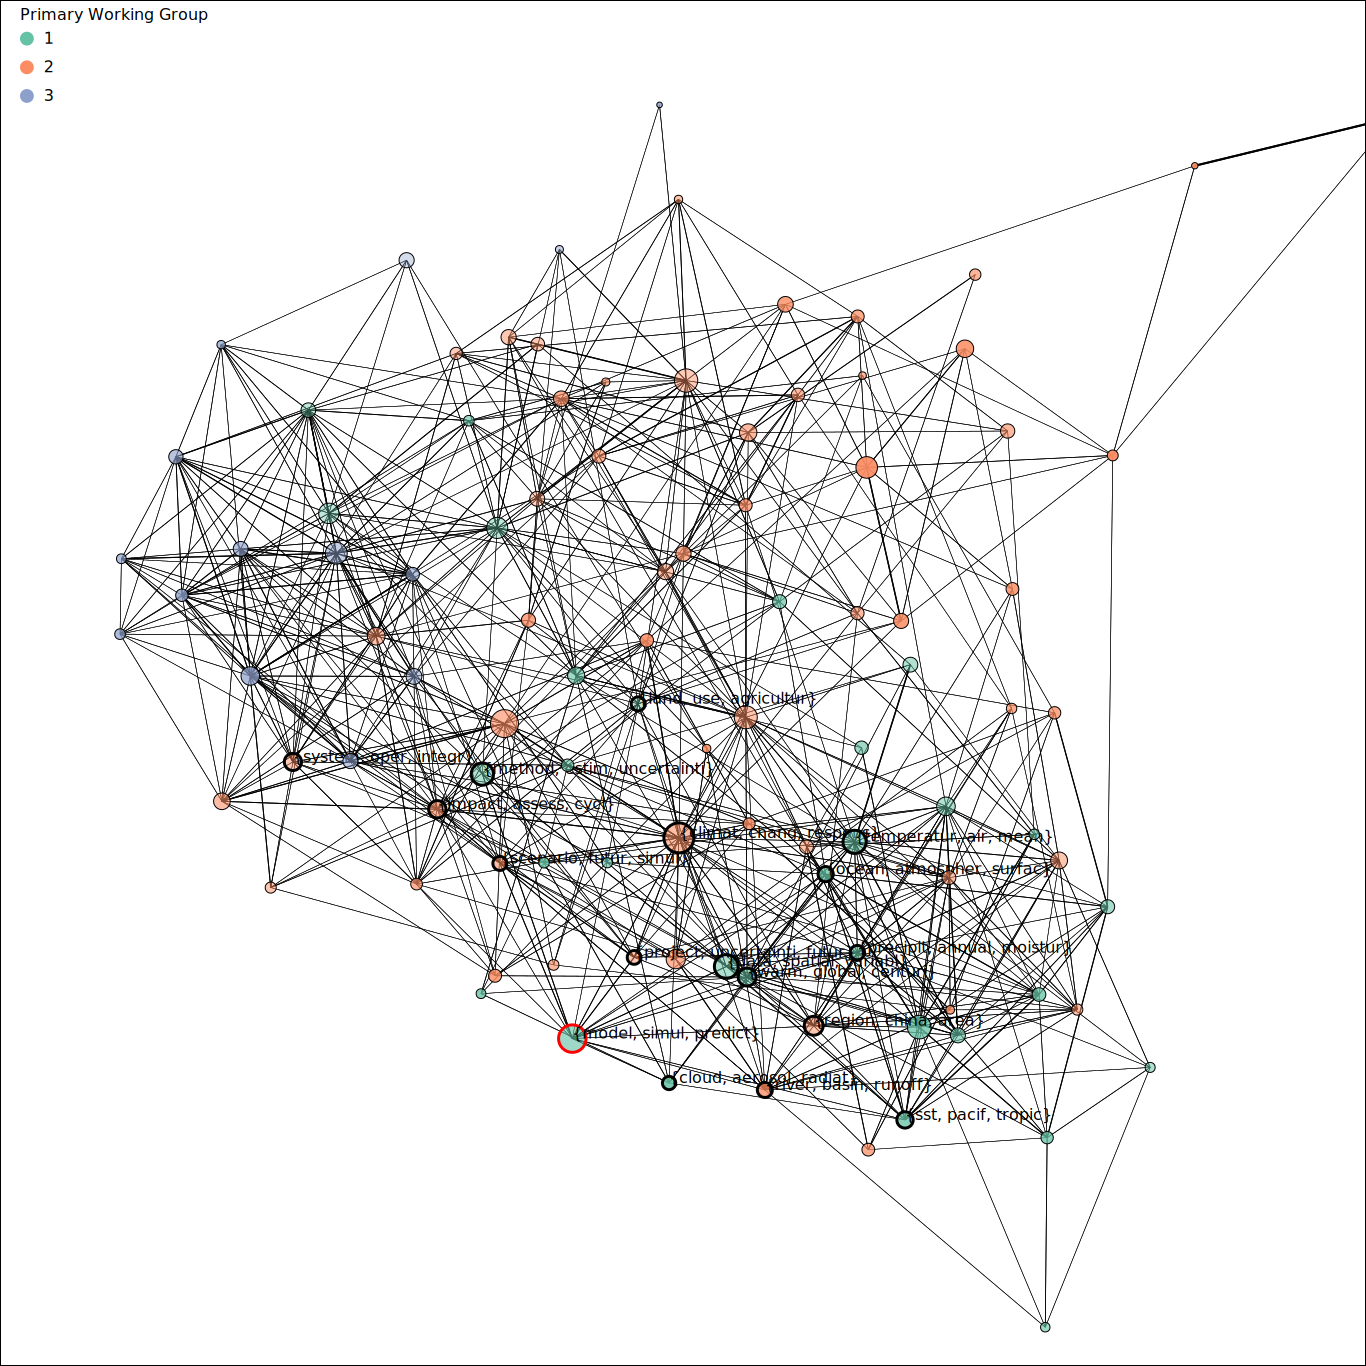
\includegraphics[width=1.1\linewidth]{../plots/network_wg_372_1.PNG}
%		\end{center}
%	\end{column}
%	\begin{column}{0.35\linewidth}
%%		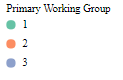
\includegraphics[width=0.4\linewidth]{../plots/network_wg_key.PNG}
%		\begin{center}
%			\begin{itemize}
%				\item The largest topic in WGI is on models.
%			\end{itemize}
%		\end{center}
%	\end{column}
%\end{columns}
%
%\end{frame}
%
%\begin{frame}{Preliminary results - structure - WGII}
%
%\begin{columns}
%	\begin{column}{0.65\linewidth}
%		\begin{center}
%			\vspace*{-0.1\linewidth}
%			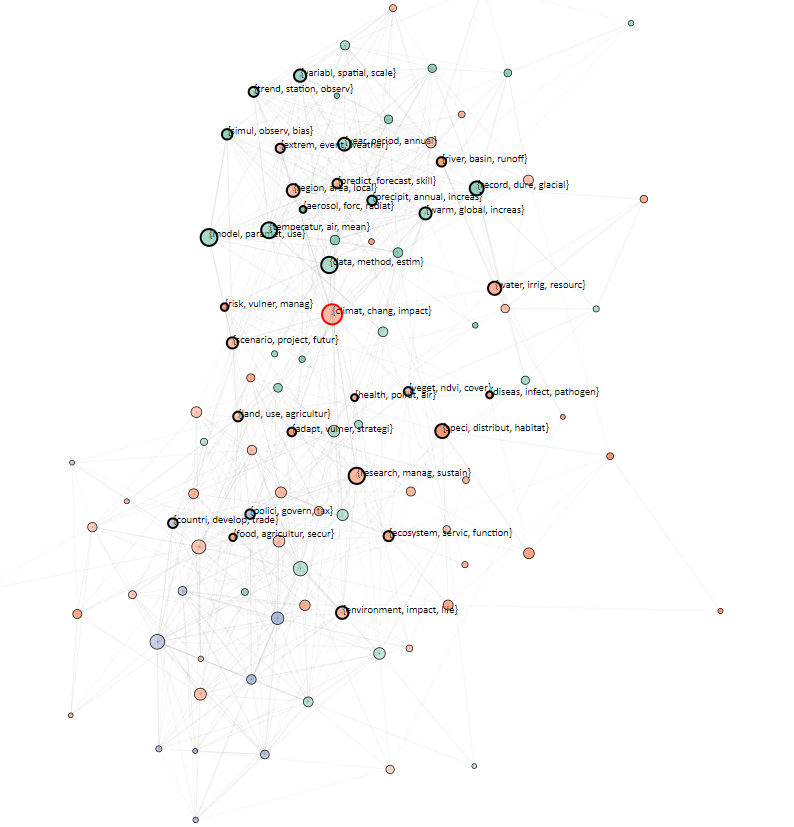
\includegraphics[width=1.1\linewidth]{../plots/network_wg_372_2}
%		\end{center}
%	\end{column}
%	\begin{column}{0.35\linewidth}
%		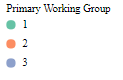
\includegraphics[width=0.4\linewidth]{../plots/network_wg_key}
%		\begin{center}
%			\begin{itemize}
%				\item The largest primarily WGII topic is on climate change impacts
%			\end{itemize}
%		\end{center}
%	\end{column}
%\end{columns}
%
%\end{frame}
%
%\begin{frame}{Preliminary results - structure - WGIII}
%
%\begin{columns}
%	\begin{column}{0.65\linewidth}
%		\begin{center}
%			\vspace*{-0.1\linewidth}
%			
\includegraphics[width=1.1\linewidth]{../plots/network_wg_372_3}
%		\end{center}
%	\end{column}
%	\begin{column}{0.35\linewidth}
%		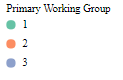
\includegraphics[width=0.4\linewidth]{../plots/network_wg_key}
%		\begin{center}
%			\begin{itemize}
%				\item The largest WGIII topic is on emissions reductions.
%			\end{itemize}
%		\end{center}
%	\end{column}
%\end{columns}
%
%\end{frame}
%
%\begin{frame}{Preliminary results - structure - other clusters}
%
%\begin{columns}
%	\begin{column}{0.65\linewidth}
%		\begin{center}
%			\vspace*{-0.1\linewidth}
%			\hspace*{-0.1\linewidth}
%			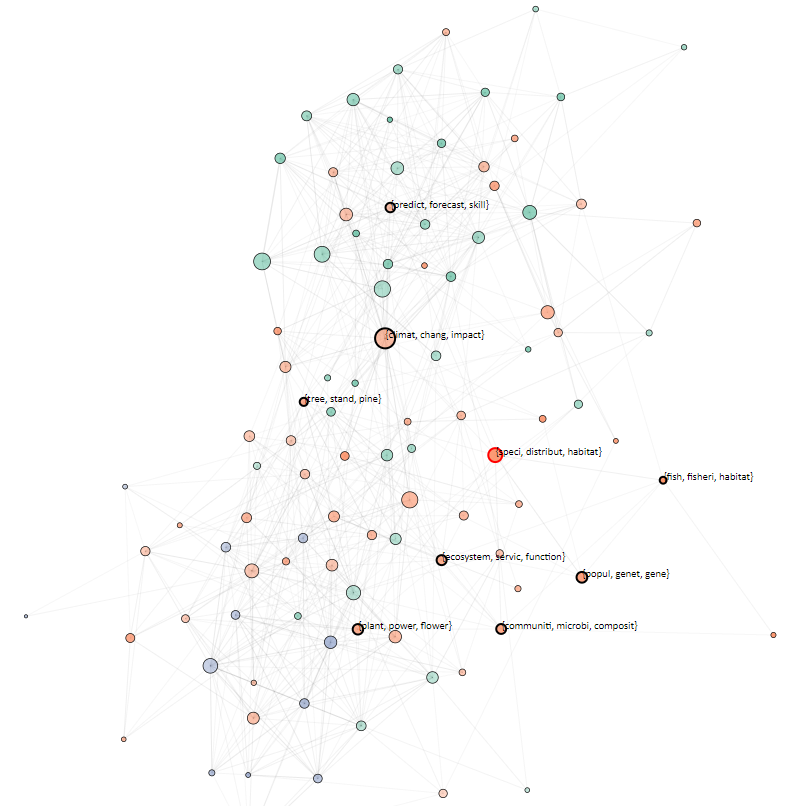
\includegraphics[width=1.25\linewidth]{../plots/network_wg_372_4}
%		\end{center}
%	\end{column}
%	\begin{column}{0.35\linewidth}
%		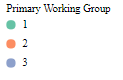
\includegraphics[width=0.4\linewidth]{../plots/network_wg_key}
%		\begin{center}
%			\begin{itemize}
%				\item A fourth cluster of mostly WGII references contains topics on ecosystems, species and habitats
%			\end{itemize}
%		\end{center}
%	\end{column}
%\end{columns}
%
%\end{frame}



%\begin{frame}{Preliminary results - structure - Sustainability}
%
%
%
%\begin{columns}
%	\begin{column}{0.6\linewidth}
%		\begin{center}			
%			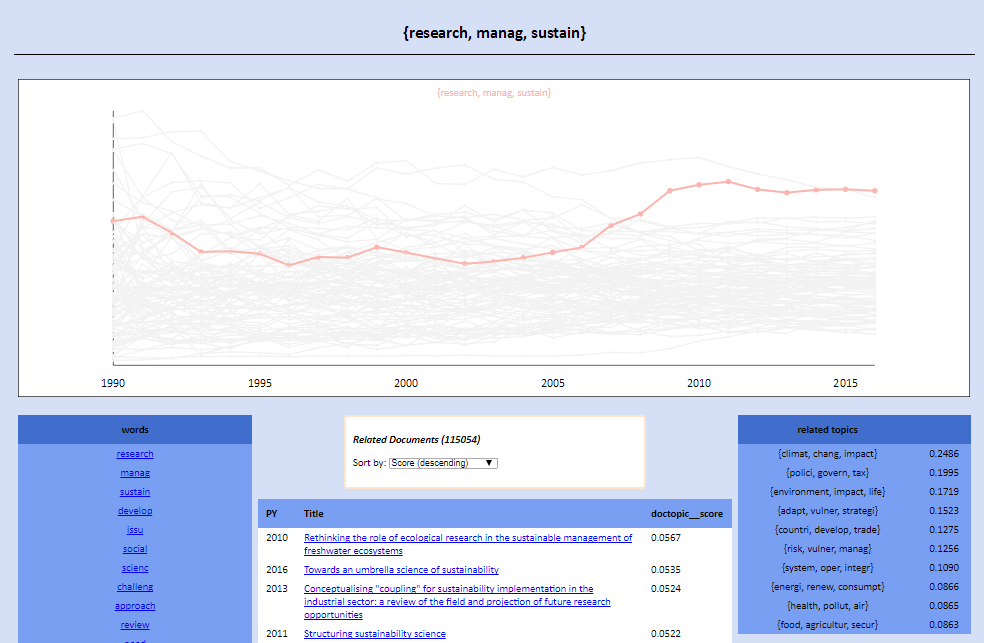
\includegraphics[width=\linewidth]{../plots/sustainability}
%		\end{center}
%	\end{column}
%	\begin{column}{0.4\linewidth}
%		\begin{center}
%			\begin{itemize}
%				\item In later assessment periods, a large meta-topic on research priorities and sustainability emerges
%			\end{itemize}
%		\end{center}
%	\end{column}
%\end{columns}
%
%\end{frame}
%
%\begin{frame}{Preliminary results - structure - Sustainability}
%
%
%
%\begin{columns}
%	\begin{column}{0.6\linewidth}
%		\begin{center}			
%			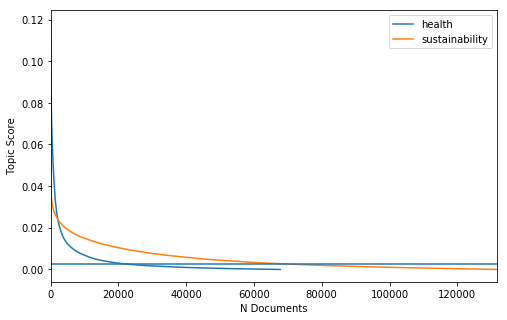
\includegraphics[width=\linewidth]{../plots/health_sustain_386}
%		\end{center}
%	\end{column}
%	\begin{column}{0.4\linewidth}
%		\begin{center}
%			\begin{itemize}
%				\item The flatness of its distribution across documents indicates a topic that occurs
%			\end{itemize}
%		\end{center}
%	\end{column}
%\end{columns}
%
%\end{frame}
%
%%% Sus table
%
%\begin{frame}{Preliminary results - structure - Sustainability}
%\begin{table}
%	\footnotesize
%	\renewcommand{\arraystretch}{2}
%\begin{tabular}{p{0.3\linewidth}p{0.3\linewidth}p{0.3\linewidth}}
%	\toprule 
%	{polici, govern, tax} & {adapt, vulner, strategi}  & {urban, citi, area} \\ 
%	\midrule 
%	How Research-Prioritization Exercises Affect Conservation Policy & Methodological choices in solution-oriented adaptation research: a diagnostic framework & A review of urban ecosystem services: six key challenges for future research  \\ 
%	Role of hydrology and economics in water management policy under increasing uncertainty & When not every response to climate change is a good one: Identifying principles for sustainable adaptation & Lines of Tradition and Recent Approaches to Urban Ecology, Focussing on Germany and the USA \\ 
%	Informing food policy: balancing the evidence & Informed adaptation: Ethical considerations for adaptation researchers and decision-makers & Advancing understanding of the complex nature of urban systems \\ 
%	The identification of priority policy options for UK nature conservation & Future oriented conservation: knowledge governance, uncertainty and learning & Sustainable urban landscapes: South African perspectives on transdisciplinary possibilities \\ 
%	Environmental education policy research challenges and ways research might cope with them & Towards an integrated agenda for adaptation research: theory, practice and policy & A conceptual framework for addressing complexity and unfolding transition dynamics when developing sustainable adaptation strategies in urban water management \\
%	\bottomrule
%\end{tabular} 
%
%\end{table}
%
%\end{frame}


%\begin{frame}{Preliminary results - growth}
%
%\begin{columns}
%	\begin{column}{0.6\linewidth}
%		\begin{center}
%			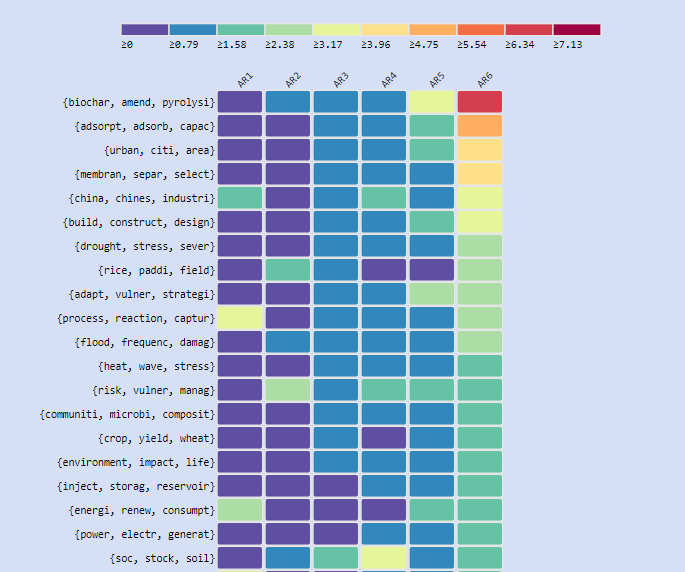
\includegraphics[width=\linewidth]{../plots/top_20_386}
%		\end{center}
%	\end{column}
%	\begin{column}{0.4\linewidth}
%		\begin{center}
%			\begin{itemize}
%				\item Negative emissions related topics have shown strong growth since the end of AR5
%				\item As have topics on cities and extreme weather events
%			\end{itemize}
%		\end{center}
%	\end{column}
%\end{columns}
%
%\end{frame}

%\begin{frame}{Preliminary results - growth - biochar}
%
%
%		\begin{center}
%			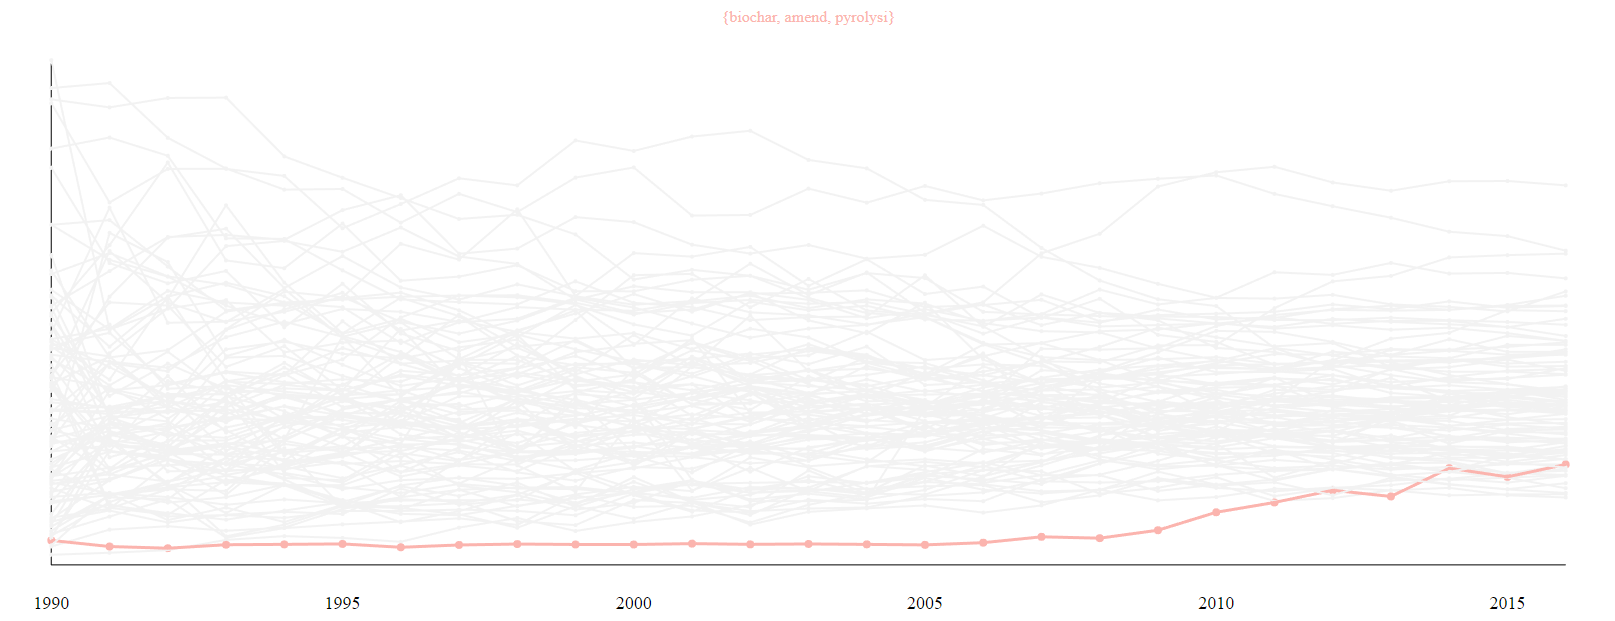
\includegraphics[width=\linewidth]{../plots/biochar_growth.png}
%
%		\medskip
%
%			\begin{itemize}
%				\item Biochar has emerged as an entirely new topic in the last 10 years
%			\end{itemize}
%		\end{center}
%
%\end{frame}

\begin{frame}{Preliminary results - gaps in coverage}

How can we get a sense of which topics are better covered in IPCC reports?

\begin{itemize}
	\item Each document \(d\) either matches or does not match an IPCC reference
	\item For each topic \(h\), we can sum the scores for each category of document
	\item The ``IPCC proportion'' of each topic is the proportion of the sum of the document score accounted for by documents which match IPCC references.
\end{itemize}



\end{frame}

\begin{frame}{Preliminary results - gaps in coverage}

\begin{columns}
	\begin{column}{0.7\linewidth}
		\begin{center}
			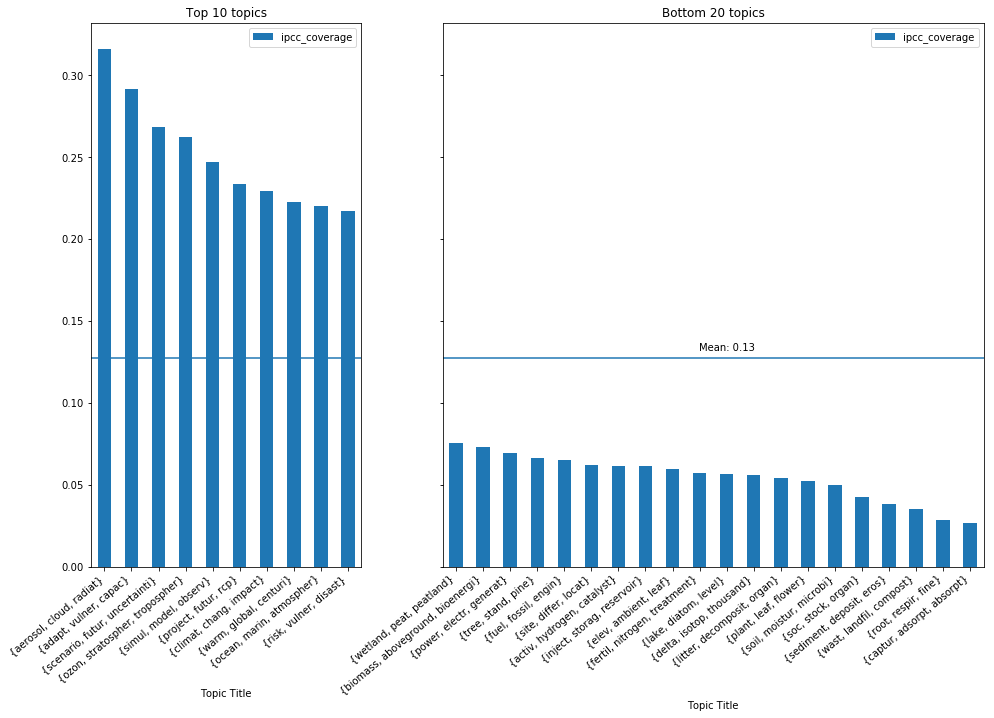
\includegraphics[width=\linewidth]{../plots/ipcc_topics_654.png}
		\end{center}
	\end{column}
	\begin{column}{0.3\linewidth}
		\begin{center}
			\begin{itemize}
				\item The physical science aspects of climate change, as well topics on impacts, adaptation and scenarios are well covered by the IPCC
				\item Topics on specific technological solutions (particularly NETs), as well as soils, are less well covered
			\end{itemize}
		\end{center}
	\end{column}
\end{columns}

\end{frame}

\begin{frame}{Preliminary results - gaps in coverage}


			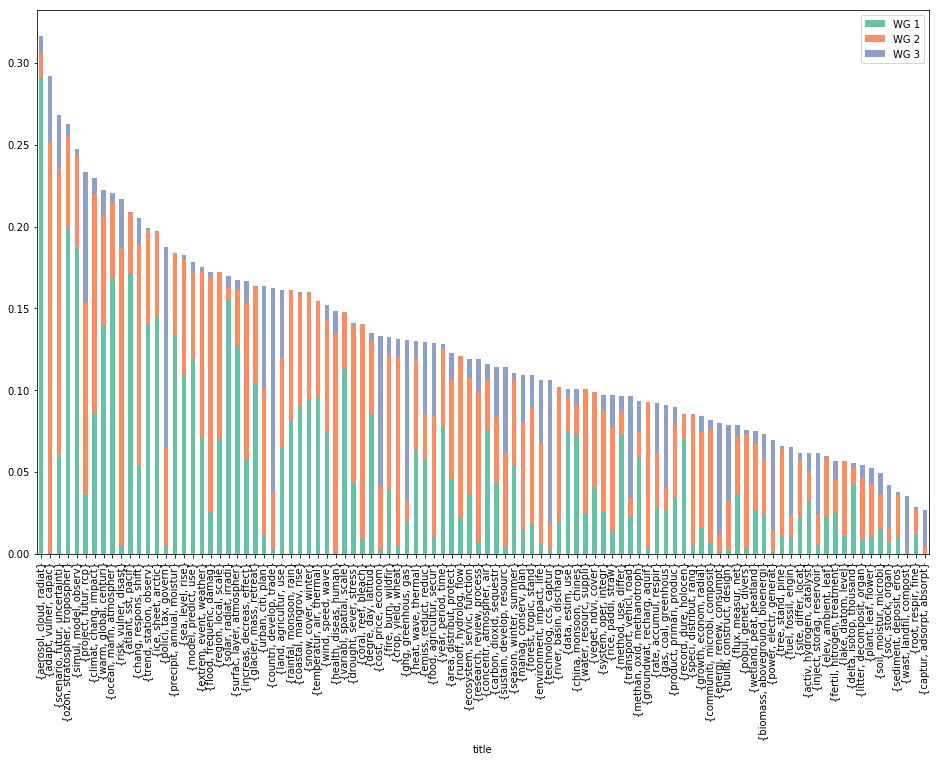
\includegraphics[width=0.8\linewidth]{../plots/ipcc_topics_wg_654.png}


\end{frame}

\begin{frame}{Preliminary results - gaps in coverage}
	
	
	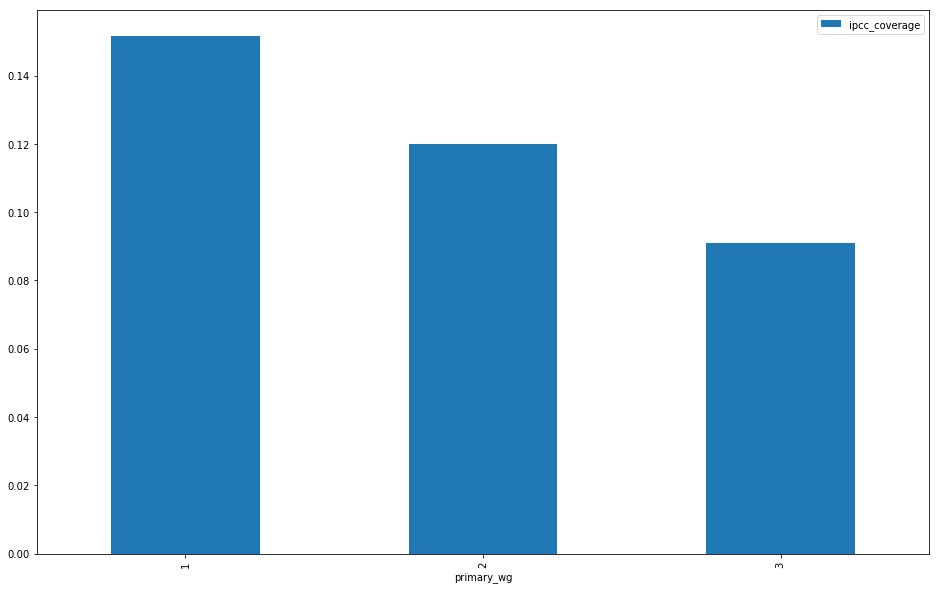
\includegraphics[width=0.8\linewidth]{../plots/ipcc_coverage_by_wg_654.png}
	
	
\end{frame}



\begin{frame}{Next steps}
	\begin{itemize}
		\item Adjusting second stage of model to give more weight to topics with many documents (to better capture emergence)
		\item Further analysis of new model
		\item (Manual) comparison of (AR6) topics with AR6 outline
	\end{itemize}
\end{frame}

%\begin{frame}{Conclusions}
%
%
%\begin{itemize}
%	\item Endogenously discovered topics make substantive sense of an unmanageable dataset of climate-relevant literature
%	\item Topic modelling discovers over-arching topics such as that on sustainability and research priorities, as well as individual, fast growing topics such as biochar or CCS
%	\item Matching documents to IPCC references, we can describe topics that belong to or bridge IPCC working groups
%	\item Quantitative evidence is found to support policy makers' dissatisfaction with a lack of `solution orientation' in IPCC reports \citep{Kowarsch2017} 
%	\item By uncovering the structure at scale of a large collection of documents, and by enabling the discovery of documents relevant to specific topics or combinations of topics, this approach can provide for more comprehensive and salient scientific assessments.
%\end{itemize}
%
%\end{frame}


%\begin{frame}{Extra results - Journals}
%
%\begin{columns}
%	\begin{column}{0.55\linewidth}
%		\begin{center}
%			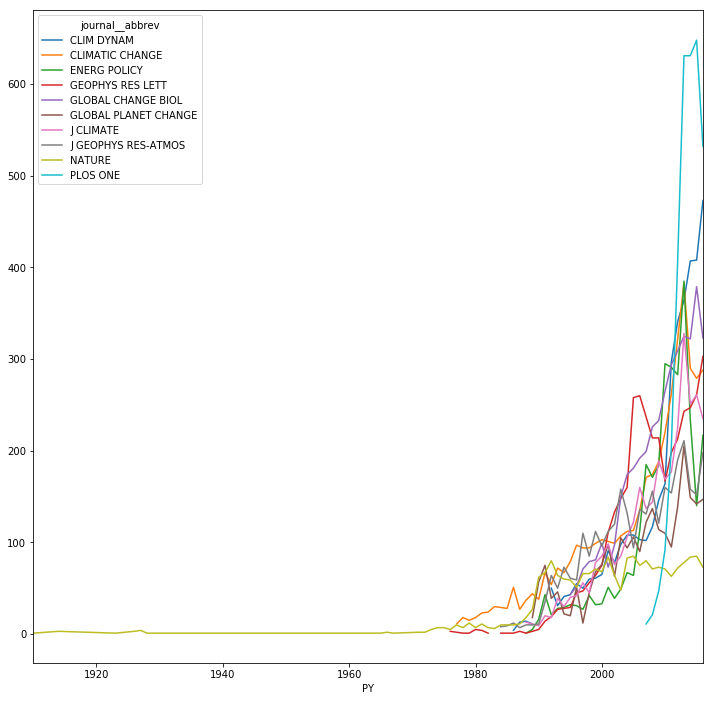
\includegraphics[width=\linewidth]{../plots/journals/journal_papers.png}
%		\end{center}
%	\end{column}
%	\begin{column}{0.45\linewidth}
%		\begin{center}
%			\begin{itemize}
%				\item Nature has been publishing about climate change for a long time
%				\item Plos One has very recently overtaken all other journals
%				\item The number of journals has risen very steeply
%			\end{itemize}
%		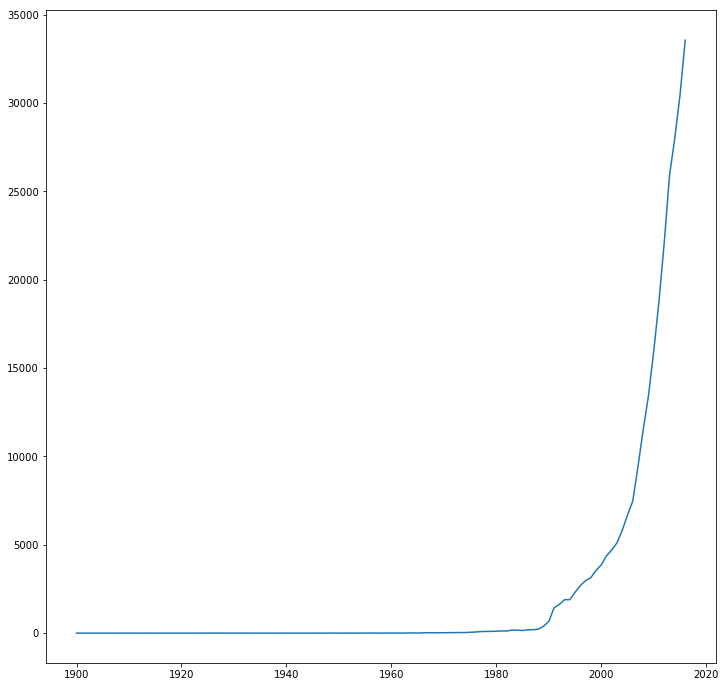
\includegraphics[width=0.9\linewidth]{../plots/journals/n_journals.png}
%		\end{center}
%	\end{column}
%\end{columns}
%
%\end{frame}

%\begin{frame}{Extra results - Journals}

%\begin{columns}
%	\begin{column}{0.55\linewidth}
%		\begin{center}
%			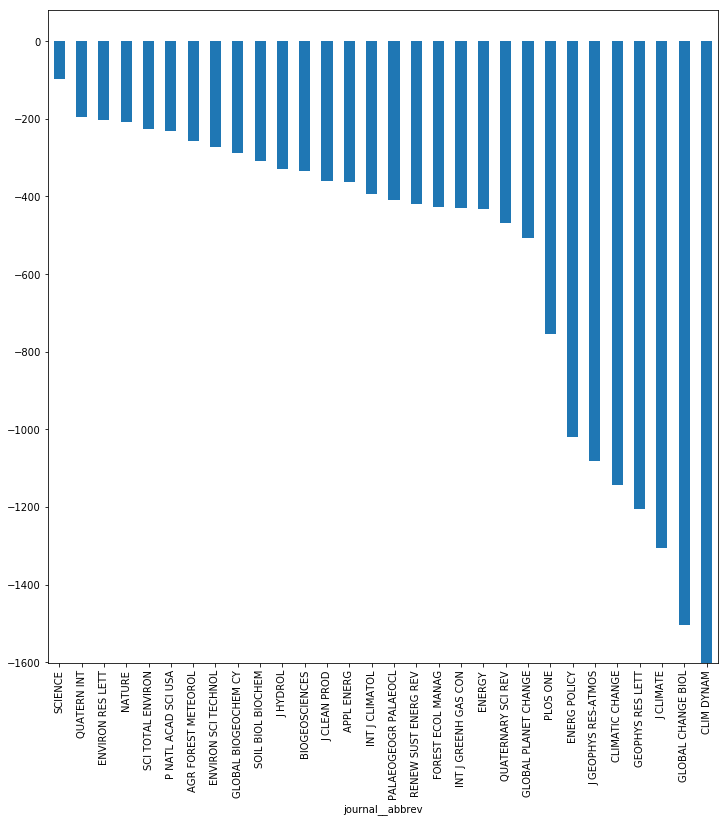
\includegraphics[width=\linewidth]{../plots/journals/journal_entropy_386.png}
%		\end{center}
%	\end{column}
%	\begin{column}{0.45\linewidth}
%		\begin{center}
%			\begin{itemize}
%				\item Journal Entropy describes the distribution of topics in a journal \citep{Hall2008a}
%				\item High values mean the journal deals with a wider range of topics
%			\end{itemize}
%			\[  H(z\rvert c,y) = -\sum_{i=1}^{K} \hat{p}(z_i \rvert c,y) \; log \; \hat{p}(z_i \rvert c, y) \]
%		\end{center}
%	\end{column}
%\end{columns}
%
%\end{frame}

%\begin{frame}{Extra results - Journals}
%
%	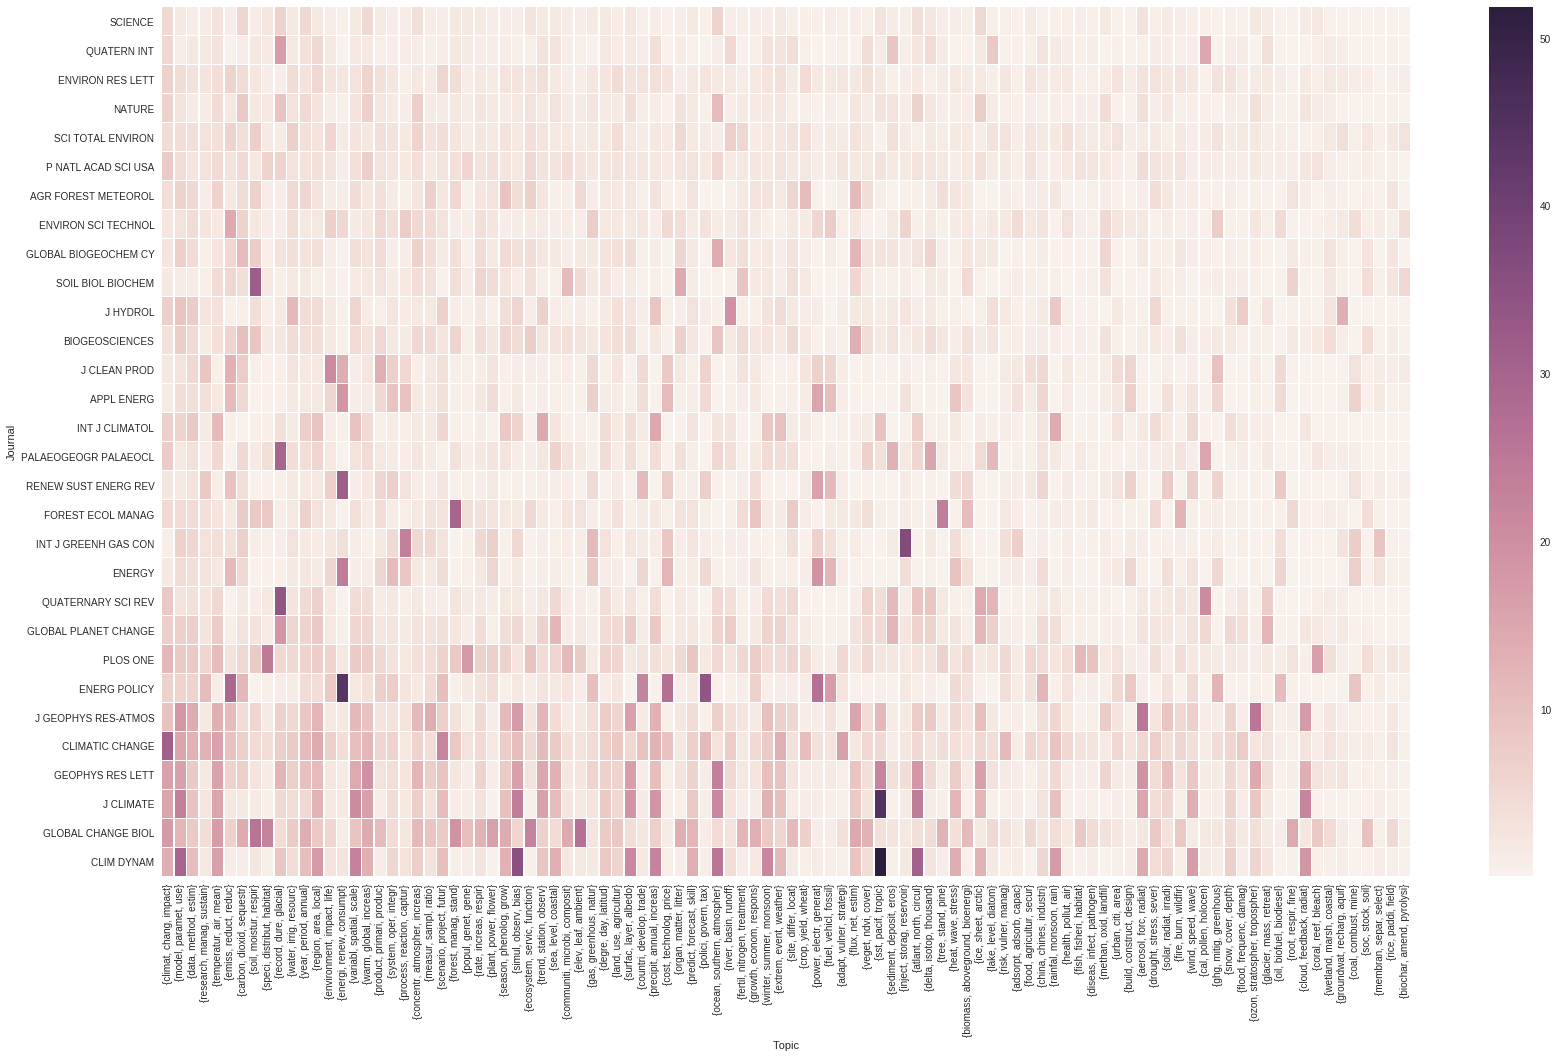
\includegraphics[width=\linewidth]{../plots/journals/journal_topics_386.png}
%
%\end{frame}


%\begin{frame}{Outlook}
%
%\begin{figure}
%
%\tiny
%
%\begin{ganttchart}[
%	y unit title=0.3cm,
%	y unit chart=0.5cm,
%	x unit= 0.2cm,
%	vgrid,hgrid,
%	vgrid={{dotted,dotted,black}},
%	title height=1,
%	%     title/.style={fill=none},
%	title label font=\bfseries\scriptsize,
%	%bar/.style={fill=blue},
%	bar height=0.7,
%	bar label font=\tiny,
%	%   progress label text={},
%	group right shift=0,
%	group top shift=0.7,
%	group height=.3,
%	group peaks width={0.2},
%	inline]{1}{42}
%	\gantttitle{2017}{9}
%	\gantttitle{2018}{12}
%	\gantttitle{2019}{12}
%	\gantttitle{2020}{9} \\
%	\gantttitlelist{2,...,4}{3} \gantttitlelist{1,...,4}{3} \gantttitlelist{1,...,4}{3} \gantttitlelist{1,...,3}{3} \\
%	\gantttitlelist{4,...,12}{1} \gantttitlelist{1,...,12}{1}
%	%\gantttitlelist{J,F,M,A,M,J,J,A,S,O,N,D}{1}
%	\gantttitlelist{1,...,12}{1} \gantttitlelist{1,...,9}{1}\\
%	
%	% HERTIE
%	\ganttgroup[inline=false]{Hertie Courses}{6}{42} \\
%	
%	\ganttbar[inline=false, bar/.append style={fill=rd}]{Research Design}{6}{15} \\
%	\ganttbar[inline=false, bar/.append style={fill=methods}]{Methods}{6}{15} \\
%	\ganttbar[inline=false, bar/.append style={fill=skills}]{Skills}{6}{15} \\
%	\ganttbar[inline=false, bar/.append style={fill=rc}]{Research Colloquium}{19}{42} \\
%	
%	% HERTIE
%	\ganttgroup[inline=false]{Thesis Research}{1}{42} \\
%	\ganttbar[inline=false, bar/.append style={fill=research}]{Knowledge Map}{1}{5} \\
%	\ganttbar[inline=false, bar/.append style={fill=research}]{Pyramid}{6}{15} \\
%	
%	
%	\ganttbar[inline=false, bar/.append style={fill=research}]{Knowledge Accumulation}{16}{27} \\
%	
%	\ganttbar[inline=false, bar/.append style={fill=research}]{Evidence in Policy}{19}{27} \\
%	
%	\ganttbar[inline=false, bar/.append style={fill=research}]{Envelope}{28}{33} \\
%	
%	\ganttbar[inline=false, bar/.append style={fill=research}]{Revisions/Contingency}{34}{42} \\
%	
%	%\ganttlinkedbar[inline=false]{Task 2}{3}{7} \ganttnewline
%	%\ganttmilestone[inline=false]{Milestone}{7} \ganttnewline
%	
%	
%	
%\end{ganttchart} 
%
%\end{figure}
%
%\end{frame}



\begin{frame}{Frame Title}
	\small
	\bibliography{../Mendeley.bib}
\end{frame}

\end{document}
